\begin{figure}[t]
\centering
\begin{tabular}{@{}c c c@{}} % @{} removes padding around the edge of the table
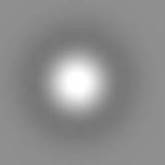
\includegraphics[width=0.2\columnwidth]{\figpath/filtering/mono_b} &
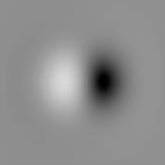
\includegraphics[width=0.2\columnwidth]{\figpath/filtering/mono_hx} &
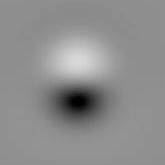
\includegraphics[width=0.2\columnwidth]{\figpath/filtering/mono_hy} \\
(a) & (b) & (c)
\end{tabular}
%
\caption{Monogenic signal filters (a) $B$, (b) $h_x$, and (c) $h_y = h_x^T$.}
\label{f:filters_monogenic}
\end{figure}